\chapter{Registers and Counters}\label{ch:registers}

\begin{objectives}
After studying this chapter you will be able to:
\begin{itemize}
  \item design registers with parallel load and shift registers, and describe serial transfer and serial addition;
  \item describe a universal shift register and write it in VHDL;
  \item explain the operation, delay and frequency limit of asynchronous (ripple) counters;
  \item design synchronous binary counters, up/down counters and counters with parallel load;
  \item build modulo-$N$ counters, including the BCD counter, and make a counter self-correcting;
  \item use ring counters and counter--decoder combinations to generate timing signals.
\end{itemize}
\end{objectives}

\section{Registers}\label{sec:registers}
A \term{register} is a group of flip-flops, each of which stores one bit. An $n$-bit register consists of $n$ flip-flops sharing one clock and stores one $n$-bit word. The simplest register (\cref{fig:reg4}) is a row of D flip-flops: at each clock edge the four inputs are copied to the outputs. Registers may also contain gates that control \emph{how} and \emph{when} new information is accepted.

\figw{403.1pt}{lect_7_4bit_register_diagram}{A 4-bit register built from D flip-flops.}{fig:reg4}

\subsection{Register with parallel load}
Transferring new information into a register is called \term{loading}; if all bits are transferred at the same moment it is a \term{parallel load}. A register that loads on every clock pulse cannot hold its data. A \emph{load} control input solves this (\cref{fig:regload}): a 2-to-1 multiplexer at each flip-flop input selects either the external data $I_i$ (when $\mathit{Load}=1$) or the flip-flop's own output (when $\mathit{Load}=0$), so that the register keeps its value through the feedback path. Equivalently, the clock may be \emph{gated}, but this is poor practice in synchronous design because it can introduce clock skew and glitches; a multiplexer (or a flip-flop with a clock-enable input) is preferred.

\figside{509.4pt}{lect_7_4bit_register_parallel_load}{A 4-bit register with parallel load. When $\mathit{Load}=0$ the flip-flops recirculate their own outputs.}{fig:regload}

\section{Shift Registers}\label{sec:shift}
A \term{shift register} can move its stored bits to the left or right. The simplest one is a chain of D flip-flops in which the output of each is connected to the input of the next and all flip-flops share a clock (\cref{fig:shift}). At each clock pulse every bit moves one position along the chain, and a new bit enters at the \emph{serial input}. Because all flip-flops change simultaneously, each captures the \emph{old} output of its neighbour, which is why the data moves exactly one position and not through the whole chain.

\figw{401.6pt}{lect_7_4bit_shift_register}{A 4-bit shift register: serial input at the left, serial output at the right.}{fig:shift}

\subsection{Serial transfer}
In a \term{serial transfer}, information is moved from a register $A$ to a register $B$ one bit at a time: the serial output of $A$ is connected to the serial input of $B$, and both registers are clocked together (\cref{fig:sertrans}). After $n$ clock pulses the $n$-bit word has been transferred. If the serial output of $A$ is also fed back to its own serial input, $A$ is \emph{rotated} and keeps its data. \Cref{tab:sertrans} traces the transfer of $A=\bin{1011}$, and \cref{fig:sertrans-timing} is the timing diagram; a serial transfer needs far fewer wires than a parallel transfer, but takes $n$ clock periods instead of one.

\begin{figure}[htbp]
\centering
\begin{subfigure}[b]{234.3pt}\centering
  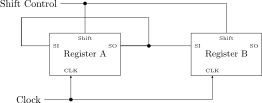
\includegraphics[width=232.3pt]{lect_7_serial_transfer}\caption{circuit}\label{fig:sertrans}
\end{subfigure}
\\[6pt]
\begin{subfigure}[b]{282.8pt}\centering
  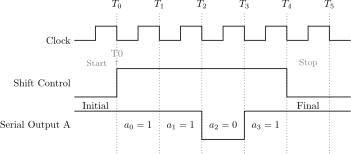
\includegraphics[width=280.8pt]{lect_7_serial_transfer_timing}\caption{timing diagram}\label{fig:sertrans-timing}
\end{subfigure}
\caption{Serial transfer from register $A$ to register $B$.}
\end{figure}

\begin{table}[htbp]
\centering
\caption{Serial transfer of $A=\bin{1011}$ into $B$ ($A$ is rotated).}
\label{tab:sertrans}
\begin{tabular}{lccc}
\toprule
Timing pulse & Serial output & Register $A$ & Register $B$\\ \midrule
Initial & --- & 1011 & 0000\\
$T_1$ & 1 & 1101 & 1000\\
$T_2$ & 1 & 1110 & 1100\\
$T_3$ & 0 & 0111 & 0110\\
$T_4$ & 1 & 1011 & 1011\\ \bottomrule
\end{tabular}
\end{table}

\subsection{Serial adder}
A \term{serial adder} adds two binary numbers one bit at a time, using one full adder instead of $n$ (\cref{fig:seradd}). Two shift registers hold the operands $A$ (augend) and $B$ (addend); at each clock pulse the least significant bits of both registers and a stored carry are added by the full adder; the sum bit is shifted into the most significant end of $A$ (so that the sum replaces the augend); $B$ is rotated to preserve its value; and the carry-out is stored in a D flip-flop for the next bit position. The flip-flop is cleared to 0 initially. \Cref{tab:seradd} traces $A=\bin{1001}$ (9) plus $B=\bin{0011}$ (3): after four pulses $A=\bin{1100}=12$. The adder is slow ($n$ clock periods) but needs very little hardware.

\figw{273.1pt}{lect_7_serial_adder}{A serial adder: one full adder and a carry flip-flop.}{fig:seradd}

\begin{table}[htbp]
\centering
\caption{Trace of the serial addition $1001+0011$.}
\label{tab:seradd}
\begin{tabular}{lcc|ccc|cc}
\toprule
Pulse & Reg.\ $A$ & Reg.\ $B$ & $x$ & $y$ & $C_{in}$ & $S$ & $C_{out}$\\ \midrule
Initial & 1001 & 0011 & --- & --- & 0 & --- & ---\\
$T_1$ & 0100 & 1001 & 1 & 1 & 0 & 0 & 1\\
$T_2$ & 0010 & 1100 & 0 & 1 & 1 & 0 & 1\\
$T_3$ & 1001 & 0110 & 0 & 0 & 1 & 1 & 0\\
$T_4$ & 1100 & 0011 & 1 & 0 & 0 & 1 & 0\\ \bottomrule
\end{tabular}

\smallskip
{\small $x$ and $y$ are the bits of $A$ and $B$ added in each step (before the shift); the registers show their contents after the pulse.}
\end{table}

\subsection{Universal shift register}
A \term{universal shift register} combines several operations in one register: clear, shift right, shift left, parallel load and no change. Two mode inputs $s_1s_0$ select the operation (\cref{tab:usr}). In the implementation (\cref{fig:usr}) a 4-to-1 multiplexer at the input of each flip-flop selects among its own output (hold), its left neighbour (shift right), its right neighbour (shift left) and the parallel input. \Cref{lst:usr} is a behavioural VHDL description: the concatenation operator \code{&} builds the shifted word, e.g.\ \code{SR_IN & reg_val(3 downto 1)} places the serial input in the MSB and drops the LSB.

\begin{table}[htbp]
\centering
\caption{Function table of a 4-bit universal shift register ($A_i^+$ is the next value of $A_i$).}
\label{tab:usr}
\begin{tabular}{cc|l|cccc}
\toprule
$s_1$&$s_0$&Operation&$A_3^+$&$A_2^+$&$A_1^+$&$A_0^+$\\ \midrule
0&0&no change&$A_3$&$A_2$&$A_1$&$A_0$\\
0&1&shift right&SIR&$A_3$&$A_2$&$A_1$\\
1&0&shift left&$A_2$&$A_1$&$A_0$&SIL\\
1&1&parallel load&$I_3$&$I_2$&$I_1$&$I_0$\\ \bottomrule
\end{tabular}
\end{table}

\begin{sidewaysfigure}[htbp]
\centering
\begin{subfigure}[b]{363.5pt}\centering
  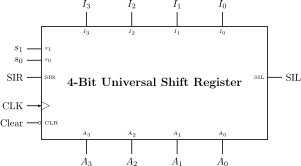
\includegraphics[width=361.5pt]{lect_7_universal_shift_register_block}\caption{block diagram}
\end{subfigure}
\caption{A 4-bit universal shift register.}\label{fig:usr}
\end{sidewaysfigure}

\begin{sidewaysfigure}[htbp]
\centering
\ContinuedFloat
\begin{subfigure}[b]{602.0pt}\centering
  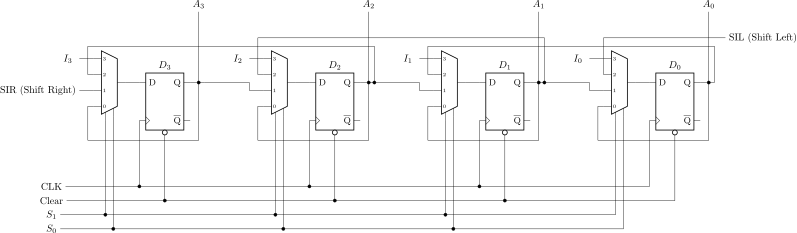
\includegraphics[width=600.0pt]{lect_7_universal_shift_register}\caption{implementation with multiplexers}
\end{subfigure}
\caption[]{A 4-bit universal shift register.}
\end{sidewaysfigure}

\vhdlfile{listings/ch07_universal_shift_register.vhd}{Behavioural VHDL of a 4-bit universal shift register with asynchronous clear.}{lst:usr}

\begin{keypoint}[Shifts are multiplications]
Shifting an unsigned binary number one place to the left multiplies it by 2 (provided no 1 is shifted out), and shifting right with a 0 entering the MSB divides it by 2 (discarding the remainder). Shifters are therefore used to multiply and divide by powers of two, and in the shift-and-add algorithms for multiplication.
\end{keypoint}

\section{Counters}\label{sec:counters}
A \term{counter} is a register that goes through a predetermined sequence of states when it is driven by input pulses, most often the clock. The sequence can be a binary count or any other. Counters are classified by how the clock reaches the flip-flops (\cref{fig:counter-block}):
\begin{itemize}
  \item in a \term{ripple} (asynchronous) counter, the output of one flip-flop clocks the next, so there is no common clock;
  \item in a \term{synchronous} counter, a common clock drives all flip-flops simultaneously.
\end{itemize}

\figw{247.9pt}{lect_7_counter_block}{General $n$-bit counter.}{fig:counter-block}

\subsection{Ripple counters}
In a \term{ripple counter} the clock is applied only to the first flip-flop, and the output of each flip-flop provides the clock of the next (\cref{fig:ripple}). Each stage is a T flip-flop with $T=1$ (a JK flip-flop with $J=K=1$), so each stage divides the frequency of its clock by 2, and the outputs form a binary count. The counter is very simple, but it is slower than a synchronous counter because the changes propagate, or ``ripple'', along the chain.

\figw{398.6pt}{lect_7_4bit_ripple_counter}{A 4-bit binary ripple counter built from T flip-flops with $T=1$.}{fig:ripple}

\paragraph{Characteristics.} The flip-flops change one after another, not together (\cref{fig:ripple-timing}).
\begin{itemize}
  \item \textbf{Propagation delay.} Each flip-flop has a delay $t_{pd}$ between a clock edge and the change of its output; in a ripple counter the delays add, so an $n$-bit counter needs up to $n\,t_{pd}$ to settle after a clock edge.
  \item \textbf{Glitches.} While the counter ripples to its final state, the outputs pass through \emph{invalid intermediate states} (for example $0111\to0110\to0100\to0000$ when counting from 7 to 8). Combinational logic or decoders connected to the outputs may see these states and produce momentary false outputs.
  \item \textbf{Frequency limit.} The next clock edge must not arrive before the previous ripple has finished: $f_{clk} < 1/(n\,t_{pd})$.
\end{itemize}
For example, a 4-bit ripple counter with $t_{pd}=10$~ns per stage settles in at most 40~ns, so the clock must be slower than 25~MHz.

\figw{243.5pt}{lect_7_4bit_ripple_counter_timing}{Timing diagram of a ripple counter: each flip-flop changes a delay after the previous one.}{fig:ripple-timing}

\subsection{BCD ripple counter}
A \term{BCD counter} counts from 0 to 9 ($\bin{0000}$ to $\bin{1001}$) and returns to 0 (\cref{fig:bcd-state}). BCD counters are essential in instruments and clocks that display decimal digits. A BCD ripple counter is obtained from the binary ripple counter by modifying two stages so that the state $1001$ is followed by $0000$ and states 10--15 are skipped (\cref{fig:bcd-ripple}).
\begin{itemize}
  \item The $J$ input of the $Q_1$ flip-flop is connected to $\overline{Q_3}$. When the count reaches $1000$ ($Q_3=1$), $J=0$ and $Q_1$ cannot toggle to 1 on the next pulse, so the sequence $1001\to1010$ never occurs.
  \item The $J$ input of the $Q_3$ flip-flop is connected to $Q_2Q_1$, so $Q_3$ sets only on the transition $0111\to1000$; $Q_3$ is reset on the transition $1001\to0000$ by its own $K=1$.
\end{itemize}

\begin{figure}[htbp]
\centering
\begin{subfigure}[b]{253.3pt}\centering
  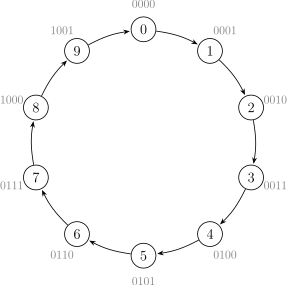
\includegraphics[width=251.3pt]{lect_7_bcd_state_diagram}\caption{state diagram}\label{fig:bcd-state}
\end{subfigure}
\\[6pt]
\begin{subfigure}[b]{412.0pt}\centering
  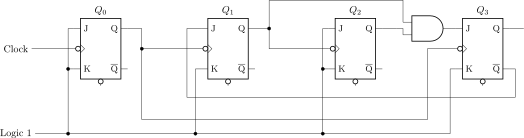
\includegraphics[width=410.0pt]{lect_7_bcd_ripple_counter}\caption{BCD ripple counter}\label{fig:bcd-ripple}
\end{subfigure}
\caption{The BCD counter.}
\end{figure}

\subsection{Synchronous binary counters}
In a \term{synchronous counter} all flip-flops are clocked together, and combinational logic at the $J$, $K$ or $T$ inputs decides which of them toggle. There is no accumulation of delays, so synchronous counters are used for high frequencies. They are designed with the standard procedure of \cref{sec:seq-design}. From the 3-bit design of \cref{ex:counter3} we know that in a binary up-counter a bit toggles when \emph{all lower-order bits are 1}:
\[
 T_{A_i} = A_{i-1}A_{i-2}\cdots A_0,\quad T_{A_0}=1 .
\]
\Cref{fig:sync} shows the 4-bit counter: the toggle condition of each stage is formed by a chain of AND gates. The delay of a synchronous counter is therefore the flip-flop delay plus the delay of one AND chain, independent of the number of bits if wider AND gates or a lookahead structure are used.

\figside{542.9pt}{lect_7_4bit_synchronous_counter}{A 4-bit synchronous binary counter with T flip-flops.}{fig:sync}

\subsection{Up/down counter}
An \term{up/down counter} counts up when $\mathit{Up}=1$ and down when $\mathit{Down}=1$ (\cref{fig:updown-state}). In the down direction a bit toggles when all lower-order bits are 0, so
\[
 T_{A_i} = \mathit{Up}\cdot A_{i-1}\cdots A_0 \;+\; \mathit{Down}\cdot \NOT{A_{i-1}}\cdots\NOT{A_0}.
\]
\Cref{fig:updown} shows the circuit.

\begin{sidewaysfigure}[htbp]
\centering
\begin{subfigure}[b]{359.5pt}\centering
  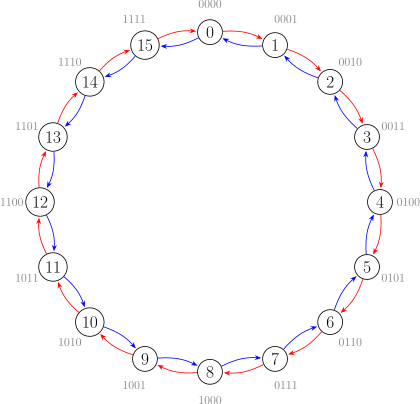
\includegraphics[width=357.5pt]{lect_7_4bit_up_down_counter_state_diagram}\caption{state diagram}\label{fig:updown-state}
\end{subfigure}
\caption{Up/down counter.}
\end{sidewaysfigure}

\begin{sidewaysfigure}[htbp]
\centering
\ContinuedFloat
\begin{subfigure}[b]{514.6pt}\centering
  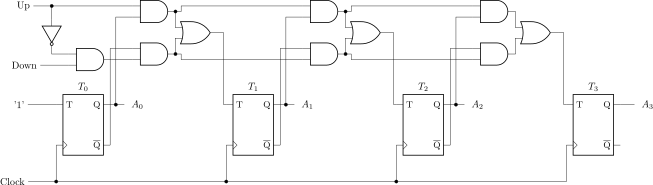
\includegraphics[width=512.6pt]{lect_7_4bit_up_down_counter}\caption{4-bit synchronous up/down counter}\label{fig:updown}
\end{subfigure}
\caption[]{Up/down counter.}
\end{sidewaysfigure}

\subsection{Counter with parallel load}
Counters in digital systems often need to be preset to a given value as well as counted. \Cref{tab:cnt-load} gives the function table of a counter with \emph{clear}, \emph{load} and \emph{count} controls (\cref{fig:cnt-load}), with a priority order: clear first, then load, then count. \Cref{lst:cnt-load} is the VHDL; the type \code{unsigned} of the package \code{numeric_std} allows the expression \code{count_val + 1}.

\begin{table}[htbp]
\centering
\caption{Function table of a 4-bit counter with parallel load (the clear is asynchronous and active-high in the VHDL of \cref{lst:cnt-load}).}
\label{tab:cnt-load}
\begin{tabular}{cccc|l}
\toprule
Clear & CLK & Load & Count & Function\\ \midrule
1 & X & X & X & clear to 0\\
0 & $\uparrow$ & 1 & X & load parallel inputs\\
0 & $\uparrow$ & 0 & 1 & count up\\
0 & $\uparrow$ & 0 & 0 & no change\\ \bottomrule
\end{tabular}
\end{table}

\figw{410.0pt}{lect_7_counter_parallel_load}{A 4-bit counter with parallel load.}{fig:cnt-load}

\vhdlfile{listings/ch07_counter_parallel_load.vhd}{VHDL of a 4-bit counter with asynchronous clear, parallel load and count enable.}{lst:cnt-load}

\subsection{Modulo-$N$ counters}
A \term{modulo-$N$ counter} goes through a repeating sequence of $N$ states and so divides the clock frequency by $N$. The BCD counter is a modulo-10 counter. A modulo-$N$ counter can be built from a binary counter with parallel load or clear in two ways (\cref{fig:bcd-load}):
\begin{itemize}
  \item \textbf{synchronous load}: detect the last count (for BCD, $9=\bin{1001}$) and, on the \emph{next clock edge}, load $\bin{0000}$; the count 9 appears for a full clock period;
  \item \textbf{asynchronous clear}: detect the first \emph{invalid} count ($10=\bin{1010}$) and clear the counter \emph{immediately}; the state 10 appears for a brief moment (a glitch) before the counter resets, which may disturb other circuits.
\end{itemize}
The synchronous method is cleaner. For BCD the detection of 9 needs only $Q_3Q_0$ since 9 is the only count between 0 and 9 with both bits 1.

\begin{figure}[htbp]
\centering
\begin{subfigure}[b]{203.7pt}\centering
  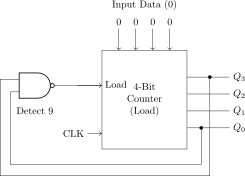
\includegraphics[width=201.7pt]{lect_7_bcd_counter_sync_load}\caption{synchronous load (detect 9)}
\end{subfigure}
\\[6pt]
\begin{subfigure}[b]{207.4pt}\centering
  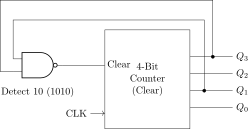
\includegraphics[width=205.4pt]{lect_7_bcd_counter_async_clear}\caption{asynchronous clear (detect 10)}
\end{subfigure}
\caption{Two ways of making a BCD counter from a binary counter,.}\label{fig:bcd-load}
\end{figure}

\figw{225.2pt}{lect_7_modulo_n_counter}{Block diagram of a modulo-$N$ counter.}{fig:modn}

\subsection{Self-correcting counters}
A counter with \emph{unused} states can enter one of them by noise or at power-up. If there is no path out of the unused states, the counter is stuck. A \term{self-correcting} design makes sure that every unused state eventually leads to a valid state. In the modulo-6 counter of \cref{fig:selfcorr} the unused states 110 and 111 both lead to 000 (\cref{tab:selfcorr}). Note that don't-cares used during minimisation must be checked afterwards: the next states of the unused states are whatever the simplified equations produce.

\begin{table}[htbp]
\centering
\caption{State table of the self-correcting modulo-6 counter.}
\label{tab:selfcorr}
\begin{tabular}{ccc|ccc}
\toprule
$Q_2$&$Q_1$&$Q_0$&$Q_2^+$&$Q_1^+$&$Q_0^+$\\ \midrule
0&0&0&0&0&1\\0&0&1&0&1&0\\0&1&0&0&1&1\\0&1&1&1&0&0\\1&0&0&1&0&1\\1&0&1&0&0&0\\ \midrule
1&1&0&0&0&0\\1&1&1&0&0&0\\ \bottomrule
\end{tabular}
\end{table}

\figw{172.8pt}{lect_7_self_correcting_counter}{State diagram of the self-correcting modulo-6 counter.}{fig:selfcorr}

\subsection{Ring counters}
A \term{ring counter} is a circular shift register in which a single 1 circulates (\cref{fig:ring}): it is initialised to $1000$ and the 1 moves one place at every pulse, producing the sequence of \cref{tab:ring}. An $n$-bit ring counter has $n$ states, and the output of each flip-flop is high for one clock period out of $n$, so the outputs are $n$ non-overlapping timing signals (\cref{fig:timing}) with no decoder needed. Each output has a frequency $f_{clk}/n$. A \term{Johnson} (twisted-ring) counter feeds back the \emph{complement} of the last output instead, which doubles the number of states to $2n$ at the cost of a decoder.

\begin{table}[htbp]
\centering
\caption{Sequence of a 4-bit ring counter.}
\label{tab:ring}
\begin{tabular}{c|cccc}
\toprule Clock & $T_0$&$T_1$&$T_2$&$T_3$\\ \midrule
$t_0$&1&0&0&0\\$t_1$&0&1&0&0\\$t_2$&0&0&1&0\\$t_3$&0&0&0&1\\$t_4$&1&0&0&0\\ \bottomrule
\end{tabular}
\end{table}

\begin{figure}[htbp]
\centering
\begin{subfigure}[b]{191.1pt}\centering
  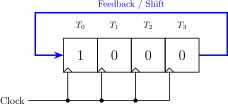
\includegraphics[width=189.1pt]{lect_7_ring_counter}\caption{4-bit ring counter}\label{fig:ring}
\end{subfigure}
\\[6pt]
\begin{subfigure}[b]{293.0pt}\centering
  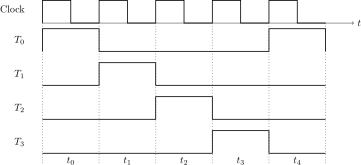
\includegraphics[width=291.0pt]{lect_7_timing_signals}\caption{timing signals}\label{fig:timing}
\end{subfigure}
\caption{Ring counter and the timing signals it generates.}
\end{figure}

\subsection{Application: generating timing signals}
Controllers need timing signals that start the successive steps of an operation. Two methods are common (\cref{fig:timing-gen}):
\begin{enumerate}
  \item a \textbf{ring counter}: $N$ flip-flops give $N$ signals directly, with no decoding, glitch-free and fast, but it needs many flip-flops;
  \item a \textbf{counter and decoder}: an $n$-bit binary counter followed by an $n$-to-$2^n$ decoder gives $N=2^n$ signals with only $n$ flip-flops, at the cost of the decoder gates (and, with a ripple counter, glitches).
\end{enumerate}
For 16 signals the ring counter needs 16 flip-flops, whereas the counter and decoder need 4 flip-flops and a 4-to-16 decoder. Timing signals of this kind drive the control unit of the processors in \cref{ch:dedicated,ch:gp}.

\begin{figure}[htbp]
\centering
\begin{subfigure}[b]{228.4pt}\centering
  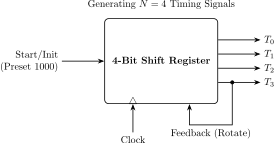
\includegraphics[width=226.4pt]{lect_7_ring_counter_generator}\caption{ring counter}
\end{subfigure}
\\[6pt]
\begin{subfigure}[b]{278.1pt}\centering
  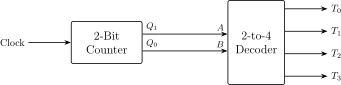
\includegraphics[width=276.1pt]{lect_7_counter_decoder_block}\caption{counter and decoder}
\end{subfigure}
\caption{Two timing-signal generators.}\label{fig:timing-gen}
\end{figure}

\begin{chaptersummary}
\begin{itemize}
  \item A \textbf{register} is a group of flip-flops; \textbf{parallel load} uses a multiplexer at each input to choose between new data and hold.
  \item A \textbf{shift register} moves its bits one place per clock; serial transfer and the \textbf{serial adder} (one full adder and a carry flip-flop) take $n$ clock periods. The \textbf{universal shift register} supports hold, shift right, shift left and load.
  \item \textbf{Ripple counters} are simple but their delays accumulate ($f_{clk}<1/(n\,t_{pd})$) and they glitch. \textbf{Synchronous counters} toggle bit $i$ when all lower bits are 1 ($T_i=A_{i-1}\cdots A_0$).
  \item \textbf{Up/down counters} combine both toggle conditions. \textbf{Counters with parallel load} can be preset and truncated: a modulo-$N$ counter uses synchronous load (detect $N-1$) or asynchronous clear (detect $N$).
  \item \textbf{Self-correcting} counters guarantee that unused states lead to a valid state.
  \item A \textbf{ring counter} generates $N$ timing signals with $N$ flip-flops; a counter with a decoder uses only $\log_2N$ flip-flops.
\end{itemize}
\end{chaptersummary}

\chapsec{Exercises}
\begin{exlist}
  \item \textbf{Register design.} Design a 4-bit register with inputs \code{CLK}, \code{CLR}, \code{LD}, \code{INC} and \code{I[3:0]}. \code{CLR = 1} resets it to \bin{0000} at the clock edge; \code{LD = 1} loads \code{I} (with priority over \code{INC}); \code{INC = 1} increments it; otherwise it holds its value. Write the behavioural VHDL.
  \item \textbf{Shift register analysis.} A 4-bit universal shift register (\cref{tab:usr}) initially holds $\bin{1010}$. Find its content after (a)~shift right with $\mathrm{SIR}=1$; then (b)~shift left with $\mathrm{SIL}=0$; then (c)~no change; then (d)~parallel load of $I=\bin{1100}$.
  \item \textbf{Counter design.} Design a synchronous modulo-6 counter (sequence 0, 1, 2, 3, 4, 5, 0, \dots) with JK flip-flops. Draw the state diagram and the excitation table, and find the $J$ and $K$ equations. Does the counter correct itself from the unused states 6 and 7?
  \item \textbf{Timing diagram.} Draw the timing diagram of a 4-bit ring counter initially in the state $\bin{1000}$ ($Q_3=1$) for five clock pulses. What is the relation between the frequency of a single output $Q_i$ and the clock frequency? How does a Johnson counter differ?
  \item Trace the serial transfer of $A=\bin{1100}$ into a register $B$ initially $\bin{0000}$ (as in \cref{tab:sertrans}), with $A$ rotating. What do $A$ and $B$ contain after four pulses?
  \item Trace the serial addition of $A=\bin{0110}$ and $B=\bin{0101}$ in the format of \cref{tab:seradd}, and give the sum.
  \item A 4-bit ripple counter uses flip-flops with $t_{pd}=10$~ns. What is the highest clock frequency, and what is the worst-case settling time when the counter changes from 0111 to 1000?
  \item Show how to use a 4-bit counter with synchronous parallel load to make a BCD counter. Give the load condition and the data inputs.
  \item Derive the $T$ input equations of a 3-bit synchronous \emph{up/down} counter with control inputs $\mathit{Up}$ and $\mathit{Down}$.
  \item You need eight timing signals. Compare (a)~a ring counter and (b)~a counter and decoder in terms of the number of flip-flops and other gates.
  \item A 4-bit universal shift register contains the unsigned number 0011 (3). What number does it hold after one shift left with $\mathrm{SIL}=0$? What is the effect on a number if the shift-left is applied $k$ times? What does a shift right with $\mathrm{SIR}=0$ do to $\bin{0110}$?
  \item Write VHDL for an 8-bit shift register with serial input \code{sin}, serial output \code{sout}, a clock and a shift-enable input \code{en}.
  \item Write the VHDL of a modulo-10 counter that counts 0--9 (4-bit output) using \code{unsigned} arithmetic and a synchronous reset to 0 after 9.
  \item Explain, with a timing sketch, how an asynchronous-clear BCD counter can produce a short glitch on the output $Q_1$ when it passes through the state 10.
\end{exlist}

\chapsec{Further Reading}
Registers and counters are covered in Chapter~6 of Mano and Ciletti~\cite{mano2018} and in Chapter~7 of Brown and Vranesic~\cite{brown2009}, which also treat Johnson counters and the VHDL of counters in more detail; see also Wakerly~\cite{wakerly2006} for the design of synchronous counters and a thorough treatment of the timing of ripple counters.
